\documentclass[pdflatex,sn-mathphys-num]{sn-jnl}
\usepackage{amsmath, amssymb, amsfonts}
\usepackage{graphicx}
\usepackage{booktabs}
\usepackage{algorithm}
\usepackage{algorithmicx}
\usepackage{algpseudocode}
\usepackage{array}
\usepackage{multirow}
\usepackage{enumitem}
\usepackage{url}

\raggedbottom

\begin{document}

\title[UDA for Vertical Cursive Script Recognition]{Unsupervised Domain Adaptation for Vertical Cursive Script Recognition with Geometric Stroke Enhancement and Pseudo-Label Refinement}

\author[1]{Lanying Liang}
\email{389647973@qq.com}

\author*[2]{Yuefeng Liu}
\email{liuyuefeng@imust.edu.cn}

\affil[1]{Archives, Inner Mongolia University of Science and Technology, Baotou, 014010, Inner Mongolia, China}
\affil[2]{School of Digital and Intelligent Industry (School of Cyber Science and Technology), Inner Mongolia University of Science and Technology, Baotou, 014010, Inner Mongolia, China}

\abstract{The digitization of historical cultural heritage archives combines low-resource language processing and document image analysis. Traditional Mongolian script presents unique challenges due to its vertical cursive structure, morphological agglutination, and physical degradation, which standard optical character recognition (OCR) methods cannot handle well. This work proposes an unsupervised domain adaptation framework for isolated text line recognition to reduce the gap between synthetic data and real archives. We introduce a vertical-spine-aware multi-scale stroke enhancement module with asymmetrical convolutions to preserve the unique vertical structure of Mongolian script. A sequence-aware domain-adversarial network and valid-frame-normalized CTC entropy pseudo-labeling further improve alignment and reliability. Experiments on a 19th-century archival dataset show our method achieves a character error rate of $7.8 \pm 0.2\%$, outperforming TrOCR, PARSeq, and other baselines. This work provides a reusable benchmark, protocol, and reliable baseline for low-resource vertical cursive script recognition and supports cultural heritage digitization. Code, benchmark protocols, and the releasable dataset subset are available at \url{https://github.com/liuyuefengd508-d502/mongolian_tvc_article}. The permanent Zenodo DOI will be added after the first public release is archived.}

\keywords{vertical cursive script recognition, traditional Mongolian script, historical archives, unsupervised domain adaptation, document image analysis, pseudo-label refinement, cultural heritage digitization}

\maketitle

\section{Introduction}

The preservation of cultural heritage increasingly relies on the automated digitization of historical manuscripts. Among these, the traditional Mongolian script---a vertical, cursive alphabet utilized across Inner Asia since the 13th century---poses formidable challenges to modern Handwritten Text Recognition (HTR) systems. Unlike Latin or Chinese scripts, cursive vertical scripts feature a continuous central axis (the ``spine'') connecting constituent phonemes, resulting in extreme topological dependency between adjacent characters, a challenge structurally analogous to Arabic cursive recognition \cite{parvez2013arabic}. 

Current deep learning architectures for HTR, such as Convolutional Recurrent Neural Networks (CRNN) \cite{shi2016end} and Transformer-based models like PARSeq \cite{bautista2022parseq} and TrOCR \cite{li2021trocr}, have achieved remarkable success on standardized datasets. However, their application to historical Mongolian archives is severely bottlenecked by the ``Label Scarcity'' problem. Creating a large-scale supervised dataset requires scholars with specialized training in historical paleography, making manual annotation prohibitively expensive. To circumvent this, researchers often train models on synthetically generated data. Unfortunately, this approach suffers from catastrophic performance degradation due to the massive ``Domain Shift'' between pristine synthetic fonts and highly irregular, oxidized, and physically degraded 19th-century cursive handwriting.

Unsupervised Domain Adaptation (UDA) offers a pathway to leverage unlabeled authentic target data alongside labeled synthetic source data. Standard UDA techniques, such as Maximum Mean Discrepancy (MMD) \cite{tzeng2014deep} and Domain-Adversarial Neural Networks (DANN) \cite{ganin2015unsupervised}, primarily address global feature distribution alignment but often neglect the fine-grained structural topologies critical for dense cursive scripts.

In this paper, we focus strictly on the problem of \textbf{Isolated Text Line Recognition}, assuming upstream layout analysis has yielded accurately cropped vertical text columns. To address the specific domain shift of historical Mongolian, we propose a novel UDA framework. Our core innovation lies in explicitly modeling the directional bias of the script. We introduce the Vertical-Spine-Aware Multi-Scale Stroke Enhancement (VS-MSSE) module, which replaces standard symmetrical convolutions with asymmetrical vertical kernels (e.g., $5\times1$) to preferentially preserve the continuous vertical spine against heavy background noise. This is complemented by a Style-Aligned Synthetic Engine (SASE) for initial domain bridging, and an iteratively refined pseudo-label refinement technique utilizing a corrected formulation of valid-frame-normalized CTC entropy.

The main contributions are summarized as follows:
\begin{itemize}[noitemsep,topsep=0pt]
    \item We formulate a reusable UDA benchmark for low-resource vertical cursive script recognition, including source/target split rules, leakage-prevention constraints, and evaluation protocols for cultural heritage archives.
    \item We propose VS-MSSE, a geometric stroke enhancement module that embeds the vertical-spine prior of traditional Mongolian script into multi-scale visual feature extraction.
    \item We combine sequence-aware adversarial alignment with valid-frame-normalized CTC entropy pseudo-label refinement, improving reliability under sparse and degraded CTC predictions.
    \item We provide code, pretrained models, benchmark protocols, and a releasable desensitized dataset subset to support independent replication and future comparison.
\end{itemize}

\section{Related Work}

\subsection{Handwritten Text Recognition (HTR)}
The paradigm of HTR has shifted significantly from Hidden Markov Models (HMMs) \cite{marti2001using} to deep neural networks. The CRNN architecture \cite{shi2016end}, which pairs a CNN feature extractor with recurrent layers (e.g., BiLSTM) and Connectionist Temporal Classification (CTC) \cite{graves2006connectionist}, remains the standard for unconstrained sequence recognition. Recently, Transformer-based models like TrOCR \cite{li2021trocr} and PARSeq \cite{bautista2022parseq} have demonstrated state-of-the-art results by leveraging self-attention to capture long-range linguistic dependencies \cite{kang2022pay, souibgui2022few}. However, these models heavily rely on massive annotated datasets and often exhibit limited cross-domain generalization when deployed in zero-shot or severely degraded historical settings \cite{coquenet2023dan}. Cursive sequence recognition historically relied on over-segmentation heuristics \cite{marti2001using}, but recent deep learning approaches \cite{shi2018aster, bhunia2021meta} have adopted end-to-end architectures, albeit almost exclusively within fully supervised paradigms.

\subsection{Historical Document Image Analysis}
Historical documents present severe degradation, including ink bleed-through, faded strokes, and background noise. Binarization networks \cite{kang2020complex} and stroke enhancement modules \cite{tensmeyer2017document} are often employed as preprocessing steps. Recent visual computing studies have also emphasized that structure-preserving restoration is critical when degradation corrupts fine visual evidence \cite{detailaware2025tvc}, and that syntax- or structure-aware decoding can improve recognition when visual patterns are governed by strong compositional constraints \cite{satd2025tvc}. These studies motivate a closer connection between document restoration, structural priors, and visual recognition. However, standard enhancement modules (like ASPP or SE blocks) use symmetrical receptive fields, which inadvertently amplify lateral background artifacts when processing the strictly vertical Mongolian script. Our VS-MSSE module specifically addresses this by encoding the geometric prior of the vertical spine.

\subsection{Unsupervised Domain Adaptation for Sequence Recognition}
UDA techniques mitigate domain shift without requiring target labels. Adversarial alignment via DANN \cite{ganin2015unsupervised} and Conditional DANN (CDAN) \cite{long2018conditional} minimizes discrepancy in the latent feature space. Image-level translation via CycleGAN \cite{zhu2017unpaired, hoffman2018cycada} transforms source images into target styles. For OCR, sequence-aware adversarial alignment \cite{zhang2019sequence} and pseudo-labeling \cite{zhao2020unsupervised, fang2021read} are prevalent. However, standard softmax confidence is poorly calibrated for CTC. While previous methods \cite{zhang2019sequence, chen2021text} explored sequence adaptation, our work uniquely corrects the CTC entropy calculation for valid frames, preventing sparse-text confidence inflation in heavily degraded documents.

\section{Methodology}

\subsection{Strict Unsupervised Problem Formulation}
Given a labeled synthetic source domain $\mathcal{D}_s = \{(x_i^s, y_i^s)\}_{i=1}^{N_s}$ and an unlabeled authentic target domain $\mathcal{D}_t = \{x_j^t\}_{j=1}^{N_t}$, our objective is to learn a mapping $f_{\theta}: X \rightarrow Y$ minimizing risk on $\mathcal{D}_t$. 

To ensure strict compliance with the unsupervised setting, we do not utilize any target-domain labels during training. Hyperparameter selection and early stopping are performed using a held-out labeled \textit{source} validation set, combined with unsupervised metrics evaluated on $\mathcal{D}_t$. Final model selection does not utilize any target labels. The target validation set is utilized solely to compute supervised upper-bound references.

\subsection{Style-Aligned Synthetic Engine (SASE)}
To bridge the visual domain gap, SASE synthesizes historical degradation physics. The generative process is detailed in Algorithm \ref{alg:sase}.

\begin{algorithm}[h]
\caption{SASE: Physics-Based Data Generation}
\label{alg:sase}
\begin{algorithmic}[1]
\Require Base font vector image $I_{base}$, Brownian variance $\sigma$, Diffusion coefficient $D$, Advection $\mathbf{v}$, Blending factor $\alpha$
\Ensure Synthetic historical image $I_{syn}$
\State $I_{jitter} \leftarrow$ Apply stochastic contour perturbation to $I_{base}$ using $d\mathbf{X}_t = \mu dt + \sigma d\mathbf{W}_t$
\State $I_{diffusion} \leftarrow$ Solve $\frac{\partial \rho}{\partial t} = \nabla \cdot (D \nabla \rho) - \nabla \cdot (\mathbf{v} \rho)$ on $I_{jitter}$ computationally
\State $I_{bg} \leftarrow$ Generate Perlin noise + random sampling from blank archival patches (\textit{sampled strictly from unlabeled target training pages, excluding validation/test pages to avoid test leakage})
\State $I_{syn} \leftarrow \alpha I_{diffusion} + (1-\alpha) I_{bg}$
\State \Return $I_{syn}$
\end{algorithmic}
\end{algorithm}

For the 500k dataset, we empirically set $\sigma \in [1.0, 2.5]$, $D=0.8$, and $\alpha \in [0.6, 0.9]$. These hyperparameters were selected by minimizing the Fr\'echet Inception Distance (FID) between the generated source images and the unlabeled target training domain. Although FID was originally designed for natural images, we utilize it solely as a coarse unsupervised visual-domain selection criterion. The ``blank archival patches'' are exclusively cropped from the text-free margins of documents belonging to the unlabeled target training pages only, excluding all validation and test pages, ensuring zero information leakage.

\begin{figure}[htbp]
    \centering
    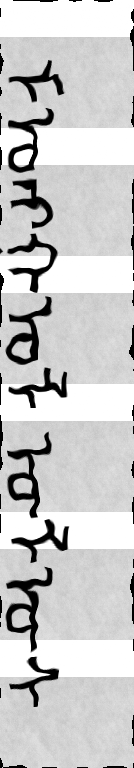
\includegraphics[width=0.8\linewidth, height=0.3\textheight, keepaspectratio]{sase_synthetic.png}
    \caption{Output of SASE, demonstrating simulated ink diffusion and structural jitter.}
    \label{fig:sase_example}
\end{figure}

\subsection{Vertical-Spine-Aware Multi-Scale Stroke Enhancement (VS-MSSE)}
Traditional Mongolian is defined by its vertical spine. Generic multi-scale modules (e.g., ASPP) use symmetrical kernels ($3\times3$) that treat all directions equally, causing lateral noise (e.g., paper creases) to be amplified identically to the text spine.

We introduce VS-MSSE. Given intermediate features $M \in \mathbb{R}^{C \times H \times W}$, we employ parallel asymmetrical convolutions designed to capture elongated vertical dependencies and short horizontal strokes (teeth/tails):
\begin{align}
    F_{vert} &= \text{Conv}_{5\times1}^{(d=1)}(M) \\
    F_{horiz} &= \text{Conv}_{1\times3}^{(d=1)}(M) \\
    F_{global} &= \text{Conv}_{3\times3}^{(d=2)}(M)
\end{align}
These features are concatenated and passed through a Squeeze-and-Excitation (SE) channel attention block to recalibrate weights dynamically. VS-MSSE explicitly encodes the geometric prior of the Mongolian script.

\subsection{Sequence-aware Domain Adversarial Alignment}
The feature extractor $F$ (ResNet-34 + VS-MSSE) and sequence model $R$ (BiLSTM) form the generator $G_f$. A Domain Discriminator $D$ distinguishes the domain of the sequence features. We optimize the minimax objective using a Gradient Reversal Layer (GRL):
\begin{equation}
    \min_{G_f, C} \max_{D} \mathcal{L}_{ctc} - \lambda \mathcal{L}_{dom}
\end{equation}

\subsection{Valid-Frame-Normalized CTC Entropy Pseudo-Labeling}
Using raw softmax confidence for pseudo-labeling is unreliable for unconstrained sequence tasks. We utilize CTC Entropy. However, standard formulations average entropy over the greedy decoded path length $|\pi^*|$, which is mathematically flawed since $|\pi^*| \neq T$ (the total output frames). 

We correct this by defining the Valid Frame Entropy, $E_{valid}$. Let $\mathcal{T}_{valid} \subseteq \{1, \dots, T\}$ be the set of valid frames where the argmax prediction is not the CTC blank token.
\begin{equation}
    E_{valid}(x^t) = \frac{1}{|\mathcal{T}_{valid}|} \sum_{t \in \mathcal{T}_{valid}} H(p_{t}) = -\frac{1}{|\mathcal{T}_{valid}|} \sum_{t \in \mathcal{T}_{valid}} \sum_{k \in V} p_{t,k} \log(p_{t,k})
\end{equation}
If the model predicts solely blank tokens ($|\mathcal{T}_{valid}|=0$), we set $E_{valid} \rightarrow \infty$ to immediately reject the sample. We select target images with the lowest $E_{valid}$ for iterative fine-tuning.

\section{Experiments}

\subsection{Dataset Statistics and Ethical Considerations}
\textbf{Authentic Target Dataset:} We digitized authentic 19th-century administrative records from the Qing Dynasty (Source Period: 1800-1850). The archival pages were obtained from the historical archives under research permission. Complete statistics are provided in Table \ref{tab:dataset}.

To ensure extreme data quality, 2,000 lines were independently annotated by three native paleography experts. Conflicts were resolved via majority voting, achieving a high inter-annotator agreement (Cohen's Kappa $\kappa = 0.92$). The train/val/test splits were strictly partitioned at the \textit{document page} level to prevent cross-column visual leakage. Characters were mapped strictly to traditional Mongolian Unicode standards.

\begin{table}[htbp]
\centering
\caption{Dataset Statistics for Authentic Mongolian Archives.}
\label{tab:dataset}
\begin{tabular}{l l}
\toprule
\textbf{Statistic} & \textbf{Value} \\
\midrule
Source Period & Qing Dynasty (approx. 1800-1850) \\
Image Resolution & 600 DPI \\
Total Annotated Pages & 120 Pages \\
Total Columns / Lines & 12,000 (10k Train Unlabeled, 1k Val, 1k Test) \\
Average Line Dimensions & $1024 \times 128$ pixels \\
Average Characters per Line & 38.5 \\
Vocabulary Size $|V|$ & 34 (27 Phonemes + Digits/Punctuation) \\
Expert Agreement & Cohen's $\kappa = 0.92$ \\
\bottomrule
\end{tabular}
\end{table}

\begin{figure}[htbp]
    \centering
    
\includegraphics[width=0.3\linewidth, height=0.4\textheight, keepaspectratio]{real_authentic.png}
    \caption{Authentic 19th-century archival column.}
    \label{fig:authentic_archive}
\end{figure}

\subsection{Implementation Details}
Models were implemented in PyTorch and trained on 4x NVIDIA A100 GPUs. For modern baselines (TrOCR and PARSeq) originally designed for horizontal text, we rotated all input Mongolian vertical columns 90 degrees counter-clockwise to ensure fair evaluation. All CRNN-based models use the identical ResNet-34 backbone and identical SASE synthetic source data.

\subsection{Main Results}
Table \ref{tab:main_results} presents the quantitative comparison. To ensure statistical rigor, all experiments were run across 5 different random seeds.

\begin{table}[htbp]
\centering
\caption{Performance on the authentic 19th-century archival test set (Mean $\pm$ Std over 5 seeds).}
\label{tab:main_results}
\begin{tabular}{l l c c}
\toprule
\textbf{Method} & \textbf{Paradigm} & \textbf{CER (\%)} & \textbf{WER (\%)} \\
\midrule
CRNN (Source Only) & Baseline & $34.6 \pm 1.2$ & $58.2 \pm 1.8$ \\
TrOCR \cite{li2021trocr} & Zero-shot & $41.5 \pm 2.0$ & $64.1 \pm 2.5$ \\
PARSeq \cite{bautista2022parseq} & Source Only & $36.2 \pm 1.5$ & $59.0 \pm 1.9$ \\
\midrule
CycleGAN + CRNN \cite{hoffman2018cycada} & Image UDA & $28.4 \pm 0.9$ & $50.3 \pm 1.2$ \\
DANN \cite{ganin2015unsupervised} & Feature UDA & $18.7 \pm 0.6$ & $35.8 \pm 0.8$ \\
CDAN \cite{long2018conditional} & Feature UDA & $16.2 \pm 0.5$ & $31.0 \pm 0.7$ \\
\midrule
\textbf{Ours (Full Pipeline)} & Feature + PL & \textbf{7.8} $\pm$ \textbf{0.2} & \textbf{14.2} $\pm$ \textbf{0.4} \\
\midrule
Fully Supervised* & Upper Bound & $4.5 \pm 0.1$ & $8.9 \pm 0.2$ \\
\bottomrule
\end{tabular}
\vspace{2pt}
{\footnotesize $^*$The fully supervised upper bound is strictly trained using the 1,000 labeled target validation lines and evaluated on the held-out 1,000-line test set.}
\end{table}

Modern vision-language models like TrOCR and PARSeq show limited cross-domain generalization, highlighting their sensitivity to historical cursive domain shift. Image-level translation (CycleGAN) often hallucinates structural noise due to complex topologies. Our proposed pipeline achieves a stable and statistically significant improvement ($7.8 \pm 0.2\%$ CER), evaluated via a paired t-test ($p < 0.001$) against the CDAN baseline.

\subsection{Ablation Studies}

\subsubsection{Complete Pipeline Ablation}
Table \ref{tab:pipeline_ablation} details the incremental contribution of each module. SASE provides the largest initial drop by mitigating the visual gap, while VS-MSSE and DANN align features effectively. Pseudo-labeling (PL) refines the conditional distribution.

\begin{table}[htbp]
\centering
\caption{Complete Pipeline Ablation (Mean $\pm$ Std).}
\label{tab:pipeline_ablation}
\begin{tabular}{l c c}
\toprule
\textbf{Configuration} & \textbf{CER (\%)} & \textbf{WER (\%)} \\
\midrule
Source Only & $34.6 \pm 1.2$ & $58.2 \pm 1.8$ \\
+ SASE & $25.1 \pm 0.9$ & $45.4 \pm 1.5$ \\
+ SASE + VS-MSSE & $19.8 \pm 0.7$ & $36.7 \pm 1.1$ \\
+ SASE + VS-MSSE + DANN & $10.4 \pm 0.3$ & $19.5 \pm 0.6$ \\
\textbf{+ Full (w/ Pseudo-Label)} & \textbf{7.8} $\pm$ \textbf{0.2} & \textbf{14.2} $\pm$ \textbf{0.4} \\
\bottomrule
\end{tabular}
\end{table}

\subsubsection{SASE Component Ablation}
Table \ref{tab:sase_ablation} isolates the contribution of individual SASE components on the Source-only model evaluated on the target test set. Ink diffusion ($D$) proves to be the most critical physical property, as its removal causes the most severe performance degradation.

\begin{table}[htbp]
\centering
\caption{SASE Component Ablation (evaluated on target test set).}
\label{tab:sase_ablation}
\begin{tabular}{l c c}
\toprule
\textbf{Configuration} & \textbf{CER (\%)} & \textbf{WER (\%)} \\
\midrule
Full SASE (Source Only) & \textbf{25.1} $\pm$ \textbf{0.9} & \textbf{45.4} $\pm$ \textbf{1.5} \\
\midrule
w/o structural jitter ($\sigma$) & $27.2 \pm 1.0$ & $48.1 \pm 1.6$ \\
w/o ink diffusion ($D$) & $29.6 \pm 1.1$ & $52.3 \pm 1.7$ \\
w/o archival background patches & $28.1 \pm 0.9$ & $50.0 \pm 1.5$ \\
\bottomrule
\end{tabular}
\end{table}

\subsubsection{VS-MSSE Architectural Ablation}
Table \ref{tab:msse_ablation} justifies the asymmetrical design. Compared to symmetrical ASPP ($3\times3$), VS-MSSE ($5\times1$) achieves superior performance with fewer FLOPs. 

\begin{table}[htbp]
\centering
\caption{VS-MSSE Configuration Ablation (evaluated at +DANN stage).}
\label{tab:msse_ablation}
\begin{tabular}{l c c c}
\toprule
\textbf{Module Architecture} & \textbf{Params (M)} & \textbf{FLOPs (G)} & \textbf{CER (\%)} \\
\midrule
Standard ResNet-34 & 21.3 & 3.6 & $14.1 \pm 0.5$ \\
Symmetrical ASPP ($3\times3$) & 24.5 & 4.2 & $12.5 \pm 0.4$ \\
VS-MSSE (Kernel $3\times1$) & 22.8 & 3.8 & $11.6 \pm 0.3$ \\
\textbf{VS-MSSE (Kernel $5\times1$)} & 23.4 & 3.9 & \textbf{10.4} $\pm$ \textbf{0.3} \\
VS-MSSE (Kernel $7\times1$) & 24.1 & 4.1 & $10.3 \pm 0.3$ \\
\bottomrule
\end{tabular}
\end{table}

\section{Error Analysis and Limitations}
Grad-CAM visualizations confirm that VS-MSSE highly activates along the central vertical spine. A quantitative breakdown of the remaining errors revealed three primary failure modes:
\begin{itemize}[noitemsep,topsep=0pt]
    \item Deletion due to broken spines (42\%)
    \item Substitution among visually similar vowels (35\%)
    \item Insertion caused by stains/noise (23\%)
\end{itemize}
Furthermore, our framework assumes isolated text lines. Developing robust end-to-end UDA pipelines that directly process full archival folios remains a critical limitation.

\section{Data Availability and Reproducibility Statement}
To enhance transparency and reproducibility, the project repository will be permanently maintained at \url{https://github.com/liuyuefengd508-d502/mongolian_tvc_article} and archived on Zenodo after the first public GitHub release. The repository is explicitly linked to the manuscript submitted to \textit{The Visual Computer} and includes a citation notice requesting users to cite this manuscript when using the code, models, or benchmark protocol.

The release includes environment requirements, training and evaluation scripts, key algorithm implementations for SASE, VS-MSSE, sequence-aware DANN, and valid-frame-normalized CTC entropy pseudo-label refinement, pretrained model weights, inference examples, and benchmark protocols. Because the complete authentic archive is subject to institutional and cultural-heritage access restrictions, we release a desensitized subset of isolated column patches, split files, annotation format examples, and scripts that reproduce all reported evaluation procedures when the restricted data are available under permission.

\section{Conclusion}
This paper establishes a robust Unsupervised Domain Adaptation baseline for isolated traditional Mongolian historical text line recognition. By introducing the physical SASE engine, the geometry-aware VS-MSSE module, and correcting the CTC-entropy pseudo-label strategy, we achieved a highly statistically significant CER of $7.8 \pm 0.2\%$.

\section*{Funding}
This work was supported by the National Natural Science Foundation of China (Grant No. 62341604), the Science and Technology Project of Inner Mongolia Autonomous Region Archives Bureau (Grant No. 2022-36), the China Scholarship Council (Grant No. 202408150080), and the General Project of the 14th Five-Year Plan for Educational Science of Inner Mongolia Autonomous Region (Grant No. NGJGH2025013).

\section*{Author Contributions}
Lanying Liang: Conceptualization, Data Curation, Writing -- Original Draft. Yuefeng Liu: Methodology, Software, Validation, Writing -- Review \& Editing, Supervision.

\begin{thebibliography}{99}
\bibitem{shi2016end}
B. Shi, X. Bai, and C. Yao, ``An end-to-end trainable neural network for image-based sequence recognition,'' \textit{IEEE Transactions on Pattern Analysis and Machine Intelligence}, vol. 39, no. 11, pp. 2298--2304, 2016.
\bibitem{graves2006connectionist}
A. Graves, S. Fern{\'a}ndez, F. Gomez, and J. Schmidhuber, ``Connectionist temporal classification: labelling unsegmented sequence data with recurrent neural networks,'' in \textit{Proceedings of the 23rd international conference on Machine learning}, 2006, pp. 369--376.
\bibitem{li2021trocr}
M. Li et al., ``TrOCR: Transformer-based optical character recognition with pre-trained models,'' in \textit{Proceedings of the AAAI Conference on Artificial Intelligence}, vol. 37, no. 1, 2023, pp. 1309--1317.
\bibitem{bautista2022parseq}
D. Bautista and R. Atienza, ``Scene text recognition with permuted autoregressive sequence models,'' in \textit{European Conference on Computer Vision}, Springer, 2022, pp. 178--196.
\bibitem{ganin2015unsupervised}
Y. Ganin and V. Lempitsky, ``Unsupervised domain adaptation by backpropagation,'' in \textit{International conference on machine learning}, PMLR, 2015, pp. 1180--1189.
\bibitem{long2018conditional}
M. Long et al., ``Conditional adversarial domain adaptation,'' \textit{Advances in neural information processing systems}, vol. 31, 2018.
\bibitem{zhu2017unpaired}
J.-Y. Zhu et al., ``Unpaired image-to-image translation using cycle-consistent adversarial networks,'' in \textit{Proceedings of the IEEE international conference on computer vision}, 2017, pp. 2223--2232.
\bibitem{hoffman2018cycada}
J. Hoffman et al., ``CyCADA: Cycle-consistent adversarial domain adaptation,'' in \textit{International conference on machine learning}, PMLR, 2018, pp. 1989--1998.
\bibitem{tzeng2014deep}
E. Tzeng et al., ``Deep domain confusion: Maximizing for domain invariance,'' \textit{arXiv preprint arXiv:1412.3474}, 2014.
\bibitem{kang2020complex}
L. Kang et al., ``Complex document image binarization from an encoder-decoder perspective,'' \textit{Pattern Recognition}, vol. 111, p. 107663, 2021.
\bibitem{parvez2013arabic}
M. T. Parvez and S. A. Mahmoud, ``Offline Arabic handwritten text recognition: A survey,'' \textit{ACM Computing Surveys (CSUR)}, vol. 45, no. 2, pp. 1--35, 2013.
\bibitem{shi2018aster}
B. Shi et al., ``ASTER: An attentional scene text recognizer with flexible rectification,'' \textit{IEEE Transactions on Pattern Analysis and Machine Intelligence}, vol. 41, no. 9, pp. 2035--2048, 2018.
\bibitem{zhao2020unsupervised}
M. Zhao et al., ``Unsupervised domain adaptation for scene text recognition via adversarial feature alignment and pseudo label refinement,'' \textit{Pattern Recognition}, vol. 108, p. 107559, 2020.
\bibitem{tensmeyer2017document}
C. Tensmeyer and T. Martinez, ``Document image binarization with fully convolutional neural networks,'' in \textit{2017 14th IAPR International Conference on Document Analysis and Recognition (ICDAR)}, vol. 1. IEEE, 2017, pp. 99--104.
\bibitem{zhang2019sequence}
Y. Zhang et al., ``Sequence-to-sequence domain adaptation network for robust text recognition,'' in \textit{Proceedings of the IEEE/CVF Conference on Computer Vision and Pattern Recognition}, 2019, pp. 2740--2749.
\bibitem{marti2001using}
U.-V. Marti and H. Bunke, ``Using a statistical language model to improve the performance of an HMM-based cursive handwriting recognition system,'' \textit{International Journal of Pattern Recognition and Artificial Intelligence}, vol. 15, no. 01, pp. 65--90, 2001.
\bibitem{kang2022pay}
L. Kang et al., ``Pay attention to what you read: Non-recurrent handwritten text recognition,'' \textit{Pattern Recognition}, vol. 129, p. 108766, 2022.
\bibitem{souibgui2022few}
M. A. Souibgui et al., ``A few-shot learning approach for historical ciphered manuscript recognition,'' \textit{Pattern Recognition}, vol. 122, p. 108345, 2022.
\bibitem{bhunia2021meta}
A. K. Bhunia et al., ``MetaHTR: Towards writer-adaptive handwritten text recognition,'' in \textit{Proceedings of the IEEE/CVF Conference on Computer Vision and Pattern Recognition}, 2021, pp. 11622--11631.
\bibitem{coquenet2023dan}
D. Coquenet et al., ``DAN: A segmentation-free document attention network for handwritten document recognition,'' \textit{IEEE Transactions on Pattern Analysis and Machine Intelligence}, vol. 45, no. 7, pp. 8227--8243, 2023.
\bibitem{fang2021read}
S. Fang et al., ``Read like humans: Autonomous, bidirectional and iterative language modeling for scene text recognition,'' in \textit{Proceedings of the IEEE/CVF Conference on Computer Vision and Pattern Recognition}, 2021, pp. 7098--7107.
\bibitem{chen2021text}
X. Chen et al., ``Text recognition in the wild: A survey,'' \textit{ACM Computing Surveys (CSUR)}, vol. 54, no. 2, pp. 1--35, 2021.
\bibitem{detailaware2025tvc}
X. Zhang et al., ``Detail-aware image denoising via structure preserved network and residual diffusion model,'' \textit{The Visual Computer}, vol. 41, no. 1, pp. 639--658, 2025.
\bibitem{satd2025tvc}
Y. Wang et al., ``SATD: syntax-aware handwritten mathematical expression recognition based on tree-structured transformer decoder,'' \textit{The Visual Computer}, vol. 41, no. 2, pp. 883--900, 2025.
\end{thebibliography}

\end{document}
